\documentclass[zavrsnirad]{../fer}
% Dodaj opciju upload za generiranje konačne verzije koja se učitava na FERWeb
% Add the option upload to generate the final version which is uploaded to FERWeb


\usepackage{blindtext}
\usepackage{subcaption}
\newtheorem{teorem}{Teorem}

%--- PODACI O RADU / THESIS INFORMATION ----------------------------------------

% Naslov na engleskom jeziku / Title in English
\title{Galjerkin finite element method}

% Naslov na hrvatskom jeziku / Title in Croatian
\naslov{Galjorkinova metoda konačnih elemenata}

% Broj rada / Thesis number
\brojrada{1884}

% Autor / Author
\author{Hrvoje Radoš}

% Mentor 
\mentor{prof. dr. sc. Tomislav Burić}

% Datum rada na engleskom jeziku / Date in English
\date{June, 2025}

% Datum rada na hrvatskom jeziku / Date in Croatian
\datum{lipanj, 2025.}

%-------------------------------------------------------------------------------


\begin{document}


% Naslovnica se automatski generira / Titlepage is automatically generated
\maketitle


%--- ZADATAK / THESIS ASSIGNMENT -----------------------------------------------

% Zadatak se ubacuje iz vanjske datoteke / Thesis assignment is included from external file
% Upiši ime PDF datoteke preuzete s FERWeb-a / Enter the filename of the PDF downloaded from FERWeb
\zadatak{Files/zadatak.pdf}


%--- ZAHVALE / ACKNOWLEDGMENT --------------------------------------------------

\begin{zahvale}
	% Ovdje upišite zahvale / Write in the acknowledgment
	Hvala na kavi...
\end{zahvale}


% Odovud započinje numeriranje stranica / Page numbering starts from here
\mainmatter


% Sadržaj se automatski generira / Table of contents is automatically generated
\tableofcontents


%--- UVOD / INTRODUCTION -------------------------------------------------------
\chapter{Uvod}
\label{pog:uvod}
Diferencijalne jednadžbe su jedan od temeljnih matematičkih
alata koji se koriste za matematičko modeliranje. Njihova
važnost se obično prvo primjeti u fizici gdje se one vrlo
intuitivno pojavljuju u područjima kao što su klasična mehanika,
elektromagnetizam, termodinamika pa i malo manje intuitivno u
područjima kao što su kvantna mehanika. Diferencijalne jednažbe
imaju velik utjecaj i na područja izvan fizike.
S njima se mogu modelirati izmjene populacija, širenje zaraza,
oblikovanje raznih genetskih obilježja (uzoraka),
širenje signala u neuronima, procesiranju slika, raznim
modeliranjima tržišta itd.
\bigskip
\\
Diferencijalne jednažbe uglavnom nije teško tumačiti. Najveći
izazov kod rada s njima je svakako traženje rješenja.
Rješenje ne mora uvijek postojati, ne mora biti jedinstveno,
a ako postoji i jedinstveno je ne mora biti moguće zapisati
ga analitički. Tim problemima se između ostaloga bavi numerička
matematika. Ovaj rad se bavi linearnim parcijalnim diferencijalnim
jednadžbama s konstantnim koeficijentima i rubnim uvjetom odnosno
traženjem njihova rješenja koristeći Galjorkinovu metodu
konačnih elemenata. Cilj rada je napraviti
C++ biblioteku koja služi kao efikasan, ali iznad svega
jednostavan alat za rješavanje PDJ-ova.
% Neki od radova koje ćemo citirati su \cite{6248073,6247753,ghiglia_pritt_phase_unwrapping,hartley2003multiple,4250461,123DCatch}.
% Trebaju nam samo radi testiranja kako izgleda referenciranje rada s konferencije, rada iz časopisa, knjige i Internetske stranice.
%
% \begin{figure}[htb]
% 	\centering
% 	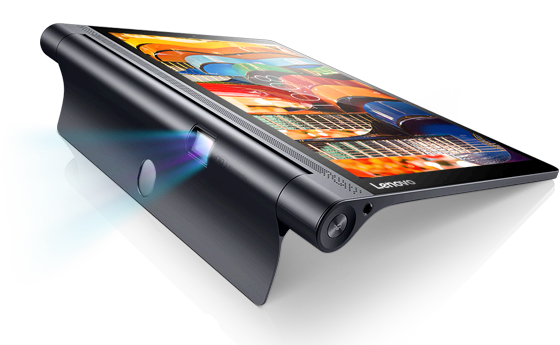
\includegraphics[width=0.38\linewidth]{Figures/lenovo_yoga_tab3_pro_front.png}
% 	\caption{Moja prva slika}
% 	\label{slk:prvaslika}
% \end{figure}
%
% Referenciramo se na sliku \ref{slk:prvaslika} u sredini rečenice, zatim prije zareza \ref{slk:prvaslika}, te zatim na kraju rečenice \ref{slk:prvaslika}.
% Upravo smo testirali radi li naredba \verb|\ref| ispravno u slučaju kada nakon nje slijedi točka.
%
% Sada slijedi jedna jednadžba:
% \begin{equation}
% 	\label{jed:prvajednadzba}
% 	\int_{-\infty}^{+\infty}f(t)\,dt=F(\omega)
% \end{equation}
% Jednadžba \eqref{jed:prvajednadzba} je moja prva jednadžba koja defnira par $f(t)\ufrek F(\omega)$ ili $F(\omega)\uvrem f(t)$.


%-------------------------------------------------------------------------------
\chapter{Glavni dio}
\label{pog:glavni_dio}
Galjorkinova metoda konačnih elemenata je složen proces
koji se sastoji od više dijelova. Na početku ovog 
poglavlja nudim kratki opis kako ovaj proces izgleda, a
u narednim poglavljima ulazim u detalje.
\bigskip
\\ 
Jednadžba koju riješavam na domeni $\Omega \subset \mathbb{R}^2$ je:

\begin{equation}
	\label{PDJ}
  A \frac{\partial^2 u}{\partial x^2}
	+ B \frac{\partial^2 u}{\partial x \partial y}
	+ C \frac{\partial^2 u}{\partial y^2}
	+ D \frac{\partial u}{\partial x}
	+ E \frac{\partial u}{\partial y}
	+ F u = f(x,y)
  \quad u \in C^2(\Omega)
\end{equation}

Ključna ideja ove metode je particioniranje domene na
što sitnije odnosno finije dijelove koje nazivamo elementima.
Takvu particiju nazivamo mesh. S meshom potom definiramo
bazne funckije koje čine bazu s kojom ćemo interpolirati
rješenje koje tražimo. Dodatnim raspisivanjem ćemo dobiti
linearni sustav čijim rješavanjem dobivamo naše traženo
rješenje.
\bigskip
\\ 
\label{uvjetNaf}
Postoji par napomena koje valja primijetiti. Ako obratimo
pažnju na jednadžbu \eqref{PDJ}, možemo primijetiti da smo
se ograničinili na rješenja iz prostora $C^2(D)$ dodatnom analizom
možemo zaključiti i da funkcija $f$ mora biti neprekinuta.
Ovo se na prvu iz perspektive primjene ne čini kao velika 
restrikcija jer nekako očekujemo da će fizikalne veličine u 
stvarnom životu uvijek biti neprekinute, ali ne samo da to nije
uvijek slučaj to jako često nije slučaj. Kao primjer navodim 
primjer djelovanja sile (npr. ovješen uteg) na nit. Za modeliranje
ovakvog sustava je potrebno opisati djelovanje te sile duž
cijelu nit, ali takav opis bi zahtijevao uporabu Diracove delta 
funkcije koja nikako nije neprekinuta, štoviše ona nije
ni funkcija nego distribucija.

\begin{figure}[htb]
	\centering
	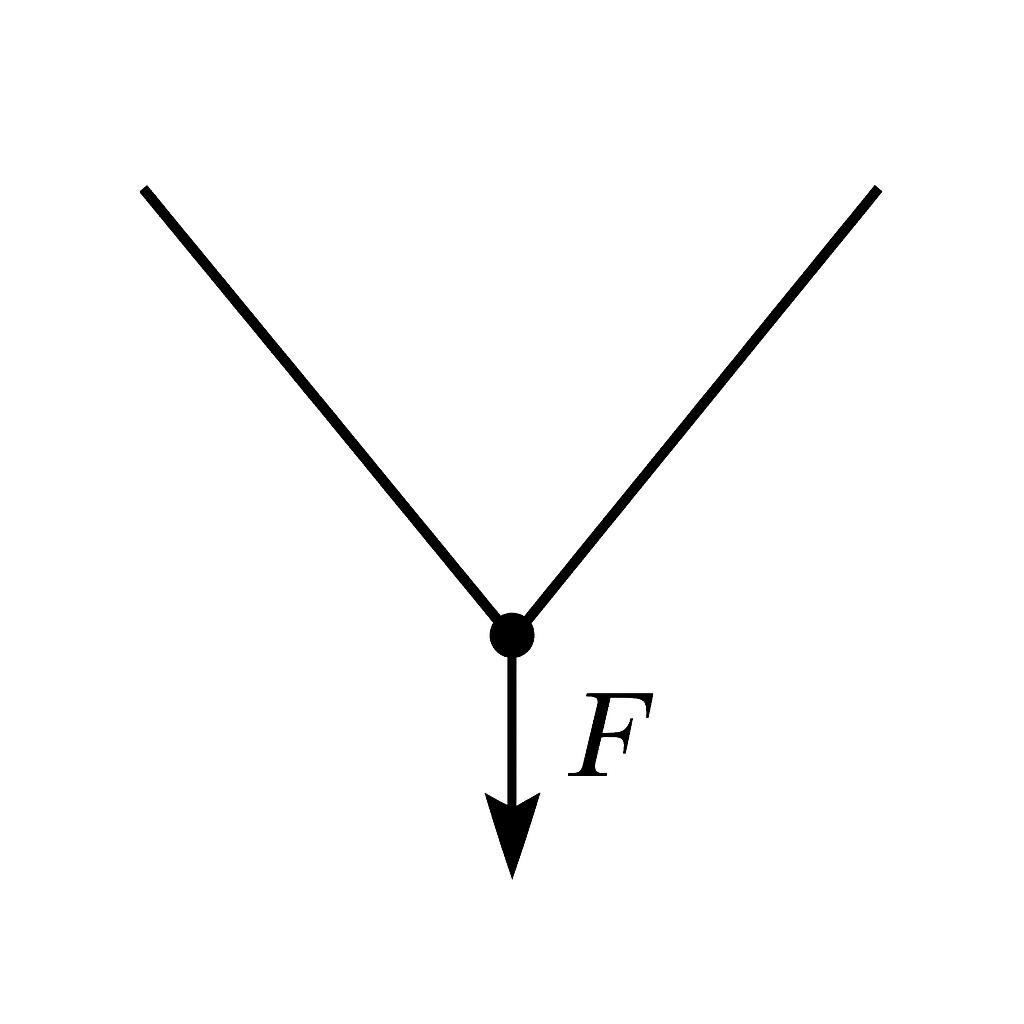
\includegraphics[width=0.38\linewidth]{Figures/nit.png}
	\caption{Djelovanje točkaste sile na nit}
	\label{nit}
\end{figure}

\section{Mesh}
\label{mesh}
Mesh je particija domene na sitne dijelove s kojima ju
možemo aproksimirati. U ovoj implementaciji ti dijelovi 
će biti trokuti (jer radimo s 2D domenom), pa ću proces
stvaranja mesha često zvati i triangulacija. S obzirom da
je jednostavnost korištenja ključno svojstvo ove implementacije 
odlučio sam se za sljedeći način unosa mesha u računalo.
\bigskip
\\ 
\textbf{Korisnik definira funkciju koja prima koordinate, a
vraća vrijednost "true" ako je točka unutar domene ili
"false" ako je točka izvan domene}
\bigskip
\\ 
Ovakav pristup omogućava da se domena definira na sličan 
način kako bi to radili na papiru iz čega proizlazi jednostavnost.
Druge C++ biblioteke za unos mesha uglavnom koriste .msh datoteke.
Ovakav pristup je dobar za komplicirane domene koje se ne mogu
lako definirati s implicitnim funkcijama, ali je presložen za neke
jednostavnije primjene. Valja napomenuti da neke biblioteke 
daju mogućnost da se domena definira preko ključnih riječi kao 
što su "circle" ili "rectangle". U usporedbi s tim rješenjima 
moj pristup daje veću fleksibilnost.
\bigskip
\\ 
Jednostavan način korištenja povlači i težinu implementacije.
Naime, kvalitetan mesh može značajno smanjiti numeričku grešku
rješenja. Naravno greška se uvijek može smanjiti tako da 
učinimo mesh finijim, ali to ne možemo raditi u nedogled.
Ova implementacija mesh generira na poprilično jednostavan način.
Za ulaz ona traži pravokutnik koji omeđuje domenu nad kojom
rješavamo PDJ. Taj pravokutnik se potom triangulira i za mesh
se uzimaju samo elementi čija su sva tri vrha unutar domene.
Ovakav pristup daje nekvalitetan mesh na rubu. Istraživajući
bolje pristupe generiranju mesha otkrio sam razne knjige koje
se bave ovom problematikom, stoga smatram da je za sada
bitno napraviti implementaciju koja se može naknadno lako 
nadograditi. Iako jednostavan pristup ovom problemu funkcionira
mislim da je bitno naglasiti gdje ova implementacija ima
mjesta za napredak.

\begin{figure}[htbp]
  \centering
  \begin{subfigure}[b]{0.45\linewidth}
    \centering
    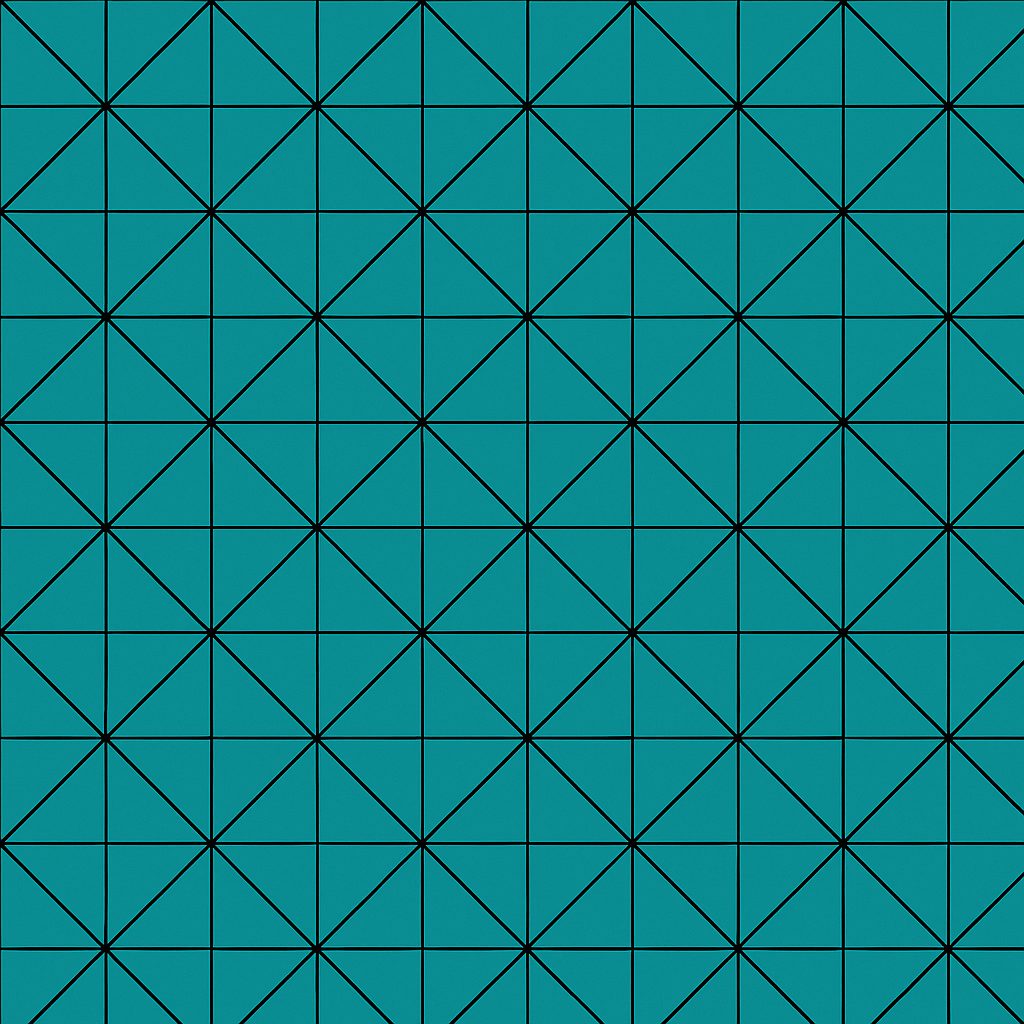
\includegraphics[width=\linewidth]{Figures/2Dmesh.png}
    \caption{Primjer 2D mesha pravokutnika}
    \label{rectMesh}
  \end{subfigure}
  \hfill
  \begin{subfigure}[b]{0.45\linewidth}
    \centering
    
\includegraphics[width=\linewidth]{Figures/apple.png}
    \caption{Složeni 3D mesh jabuke}
    \label{jabuka}
  \end{subfigure}
  \caption{Primjeri mesheva}
  \label{meshevi}
\end{figure}

\subsection{Bazne funkcije}

Nakon uspješno generiranog mesha je potrebno definirati
bazne funkcije. Bazne fukcije ćemo definirati tako da
na svakom elementu definiramo polinom prvog stupnja koji
iznosi $1$ iznad jednog vrha, a $0$ iznad ostalih \ref{baznaFja}
\begin{figure}[htb]
	\centering
	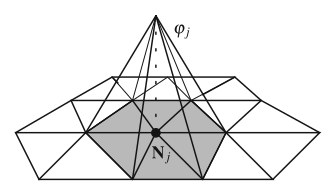
\includegraphics[width=0.5\linewidth]{Figures/baznaFja.png}
	\caption{bazna fukcija za neki čvor $j$}
	\label{baznaFja}
\end{figure}
Ovo ćemo napraviti za svaki čvor. 
\bigskip
\\ 
Kada budemo radili račun kao što su numerička integracija i 
slično nad elementima bit će od velike koristi transformirati
koordinate tako da element koji trenutno računamo postane 
oblika pravokutnog trokuta s vrhovima u $(0,0)$,$(1,0)$,$(0,1)$.
Neka su $(X_0, Y_0)$,$(X_1, Y_1)$,$(X_2, Y_2)$ vrhovi elementa
kojeg želimo preslikati. Supsitucija $(x, y) \rightarrow (\hat x, \hat y)$
je dana s:
\begin{align}
  x = (X_1 - X_0)\hat x + (X_2 - X_0)\hat y + X_0 \\ 
  y = (Y_1 - Y_0)\hat x +(Y_2 - Y_0) \hat y + Y_0
\end{align}


\section{Slaba formulacija problema}
\label{slabaFormulacija}
Radi daljne analize potrebno je navesti jedan bitan 
teorem.
\\ 
\begin{teorem}[Pravilo za divergenciju produkta]
\label{tm1}
Neka je $\Omega \subset \mathbb{R}^n$ omeđen otvoreni
skup s komadno glatkom granicom $\Gamma = \partial \Omega$,
te neka su $u : \Omega \to \mathbb{R}$ i $\mathbf{V} : \Omega \to \mathbb{R}^n$ 
dovoljne regularnosti odnosno $\partial \Omega$ je
Lipschitz neprekinuta, a $u,v \in H^1(\Omega)$
. Tada vrijedi:
\[
\int_{\Gamma} u \mathbf{V} \cdot \hat{\mathbf{n}} \, d\Gamma = 
\int_{\Omega} u \, \nabla \cdot \mathbf{V} \, d\Omega + 
\int_{\Omega} \nabla u \cdot \mathbf{V} \, d\Omega.
\]
\end{teorem}
\textbf{Napomena:} $H^1(\Omega)$ označava Soboljev prostor.
\bigskip
\\ 
Vratimo se sada na \ref{PDJ}.
Cilj nam je dobiti njezinu takozvanu slabu formulaciju.
Prvo ćemo reformularti PDJ. Primijetimo da vrijedi:
$$\nabla \cdot (A \nabla u) = 
  A \frac{\partial^2 u}{\partial x^2}
	+ B \frac{\partial^2 u}{\partial x \partial y}
	+ C \frac{\partial^2 u}{\partial y^2}
$$
Gdje:
$$A = 
\begin{pmatrix}
  A & B \\ 
  0 & C
\end{pmatrix}
 $$
 Također vrijedi:
 $$ \nabla u \cdot a =
 D \frac{\partial u}{\partial x}
	+ E \frac{\partial u}{\partial y} $$

Gdje:
$$a = 
\begin{pmatrix}
  D\\ 
  E
\end{pmatrix}
$$
Time dobivamo sljedeću jednadžbu:
\begin{equation}
  \label{vektorVerzija}
\nabla \cdot (A \nabla u)  + \nabla u \cdot a + Fu = f(x,y)
\end{equation}
Do slabe formulacije dolazimo tako da obje strane \ref{vektorVerzija} 
pomnožimo
s baznom funkcijom $\varphi_i$, integriramo po $\Omega$
i onda primijenimo  \ref{tm1} 
imamo:
\begin{equation}
  \int_{\Omega}\nabla \cdot (A \nabla u) \varphi_i \, d\Omega  + 
  \int_{\Omega} \nabla u \cdot a\varphi_i \, d\Omega  + F\int_{\Omega}u\varphi_i\,d\Omega  =
  \int_{\Omega}f(x,y)\varphi_i \, d\Omega 
\end{equation}
Primjenom teorema \ref{tm1} 
dobije se:
\begin{equation}
  \label{kobasica}
  \int_{\partial \Omega}(A \nabla u) \varphi_i \, d\Gamma  - 
  \int_{\Omega}(A \nabla u) \cdot \nabla \varphi_i \, d\Omega  + 
  \int_{\Omega} \nabla u \cdot a\varphi_i \, d\Omega  + F\int_{\Omega}u\varphi_i\,d\Omega  =
  \int_{\Omega}f(x,y)\varphi_i \, d\Omega 
\end{equation}
S obzirom da su funkcije $\varphi_i$ po definiciji
na rubu jednake $0$, jednadžba 
\ref{kobasica} se 
svede na:
\begin{equation}
  \label{slabaFor}
  -\int_{\Omega}(A \nabla u) \cdot \nabla \varphi_i \, d\Omega  + 
  \int_{\Omega} \nabla u \cdot a\varphi_i \, d\Omega  + F\int_{\Omega}u\varphi_i\,d\Omega  =
  \int_{\Omega}f(x,y)\varphi_i \, d\Omega 
\end{equation}
Primijetimo kako u ovakvom obliku funkcija $f(x,y)$ 
na sebi ima puno lakše uvjete (Sjetimo se \ref{uvjetNaf})
\bigskip
\\
Sada interpolacijom:
$$u = \sum_{j=0}^N \alpha_j \varphi_j$$
dobivamo sustav:
\begin{equation}
\label{linSustav}
A x = b
\end{equation}
Gdje:
$$(A)_{i,j} = \int_{\Omega} (A\nabla \varphi_j) \cdot \nabla \varphi_i \, d\Omega + 
\int_{\Omega} (\nabla \varphi_j \cdot a) \varphi_i \, d\Omega +
F \int_{\Omega} \varphi_j \varphi_i \, d\Omega$$
$$b_i = \int_{\Omega} f(x,y) \varphi_i \, d \Omega$$

Naime ovaj postupak vrijedi samo s Dirichletovim
rubnim uvjetima. Neka su čvorovi mesha na rubu indeksirani
od $N+1$ do $N_b$.
Kada bi se rješenje na rubu ponašalo kao
$R(x,y)$ gdje $R(x,y) = \sum_{j=N + 1}^{N_b} g_j \varphi_j$,
onda bi morali napraviti sljedeću
supsituciju:
$$u = \overset{\circ}u + R$$
Sustav \ref{linSustav}
postaje:
$$Ax = b - r$$
gdje je:
$$r_i = - \int_{\Omega}(A\nabla R) \nabla \varphi_i \, d \Omega +
\int_{\Omega}(\nabla R \cdot a) \varphi_i \, d \Omega +
F \int_{\Omega} R \varphi_i\, d\Omega
$$
Time smo problem rješavanja PDJ sveli na problem
rješavanja linearnog sustava.
%napiši opet isto, ali za rubni uvjet
%eventualno možeš pričati o proširenjima za vrijeme

\section{Postojanje rješenja}
\label{postojanje}
%Lax Milgram
Iako se možda na prvi pogled čini da smo gotovi, potrebno 
je vidjeti da rješenje uopće postoji, stoga uvodim 
Lax-Milgramov teorem.
\begin{teorem}
  \label{laxMil}
Neka je $ V $ Hilbertov prostor i neka je $ a: V \times V \rightarrow \mathbb{R} $ bilinearna forma koja zadovoljava:
\begin{itemize}
    \item \textbf{Kontinuitet:} postoji konstanta $ C > 0 $ takva da
    $$
    |a(u, v)| \leq C \|u\|_V \|v\|_V \quad \text{za sve } u, v \in V.
    $$
    
    \item \textbf{Koercivnost (eliptičnost):} postoji konstanta $ \alpha > 0 $ takva da
    $$
    a(v, v) \geq \alpha \|v\|_V^2 \quad \text{za sve } v \in V.
    $$
\end{itemize}

Tada za svaki linearni funkcional $ f \in V' $ postoji jedinstveno $ u \in V $ takvo da:
$$
a(u, v) = f(v) \quad \text{za sve } v \in V.
$$
\end{teorem}
Lako se vidi da se naš sustav \ref{linSustav} 
može svesti na problem s linearnim funkcionalima iz
\ref{laxMil}. Iz toga se lako zaključuje da
postojanje rješenja možemo garantirati samo za ispravan mesh
(to garantira implementacija) i za eliptičke PDJ što se lako provjeri programski.

\section{Implementacijski detalji}
\label{implementacijaOpis}

\subsection{CSR oblik matrice}
\subsection{Rješavanje sustava}
\subsection{Reprezentacija mesha u računalu}
%-------------------------------------------------------------------------------
\chapter{Rezultati i rasprava}
\label{pog:rezultati_i_rasprava}



%--- ZAKLJUČAK / CONCLUSION ----------------------------------------------------
\chapter{Zaključak}
\label{pog:zakljucak}



%--- LITERATURA / REFERENCES ---------------------------------------------------

% Literatura se automatski generira iz zadane .bib datoteke / References are automatically generated from the supplied .bib file
% Upiši ime BibTeX datoteke bez .bib nastavka / Enter the name of the BibTeX file without .bib extension
\bibliography{literatura}



%--- SAŽETAK / ABSTRACT --------------------------------------------------------

% Sažetak na hrvatskom
\begin{sazetak}
	Unesite sažetak na hrvatskom.

\end{sazetak}

\begin{kljucnerijeci}
	prva ključna riječ; druga ključna riječ; treća ključna riječ
\end{kljucnerijeci}


% Abstract in English
\begin{abstract}
	Enter the abstract in English.

\end{abstract}

\begin{keywords}
	the first keyword; the second keyword; the third keyword
\end{keywords}


%--- PRIVITCI / APPENDIX -------------------------------------------------------

% Sva poglavlja koja slijede će biti označena slovom i riječi privitak / All following chapters will be denoted with an appendix and a letter
\backmatter

\chapter{The Code}



\end{document}
